

\chapter{ASIC Design Flow}

%\subsection{Overview}



Since the main purpose of this work is the design of blocks concerning an Application Specific Integrated Circuit \ac{asic}, an overview of the design process is presented in this section. %before delving into implementation issues concerning the MR-OFDM mode of the IEEE802.15.4g.%, the design flow also show key stages that can affect the design. 

ASICs are custom made integrated circuits intended to perform specific tasks. A Bitcoin Miner a Radio Frequency Identification (RFID), transceivers or audio processing chips are all examples of ASICs. Design, test and evaluation of ASICs are very complex tasks. Three main variables dictates the constraints in the design process: 

\begin{enumerate}
\item \textit{Speed}: as in speed of operation, i.e. how fast the chip can perform its computations.
\item \textit{Area}: in how much the design can occupy in terms of logic gates or transistors, since occupied area means manufacturing costs and portability.
\item \textit{Power}: in how much power is consumed, since much of these devices are designed to operate in mobile applications that depends on battery, and due to heating problems caused by power dissipation. 
\end{enumerate}

 
%also power is of concern due to

ASIC design can be classified into two major categories: Digital Design, where circuits that use a great number of standard pre-designed standard cells that describe basic logic functions (as in \emph{and}, \emph{or} gates for example) are employed. Digital circuits can employ millions of those standard cells. On the other hand, analog circuits, the second major category of ASIC circuits, use a smaller number of cells. Analog circuits are custom made, use different voltage levels and much less transistors than digital circuits. Amplifiers, mixers and Voltage Controlled Oscillators are all examples of analog circuit implementations, while digital circuits implementations include, decoders, correlators, digital filters, communication protocols, routing algorithms. The review of the design flow presented in this chapter is only concerned with the digital design flow. 

%The design flow can be divided into two main parts, front end design, where system requirements are defined as well as architectures definitions, RTL design and logic verification. Back end design, that involves more physical related tasks, as distributions of circuits in the chip, connections between components, power distribution, the back end process is closely related to the technology used while the front end is typically technology independent. Another important division in ASIC design is the circuit type used, analog and digital circuits are employed depending on the applications. Digital designs use a great number of standard pre-designed cells, that contains the digital logic functions, \emph{and} \emph{or} gates etc. On the other hand, analog circuits are custom made, may use different voltage levels, fewer transistor. The review presented in this section concerns only the digital part.  




Figure~\ref{fig:asic_flow} shows the basic ASIC design flow. The first stage of the digital design process is the functional specification. It comprises a description of the system, application, requirements, as well as design constraints. The constraints are derived for the intended application and are based on the three key parameters mentioned before: power, area and speed. E.g. low power designs with low area consumption are the adopted approach for mobile applications, since this kind of application are often powered by batteries. After specifications analysis and constraints definitions, models are developed. Fixed or floating point behavioral models, described in a high level language, validate the functional specification.



\begin{figure}[hbt]
  \centering
    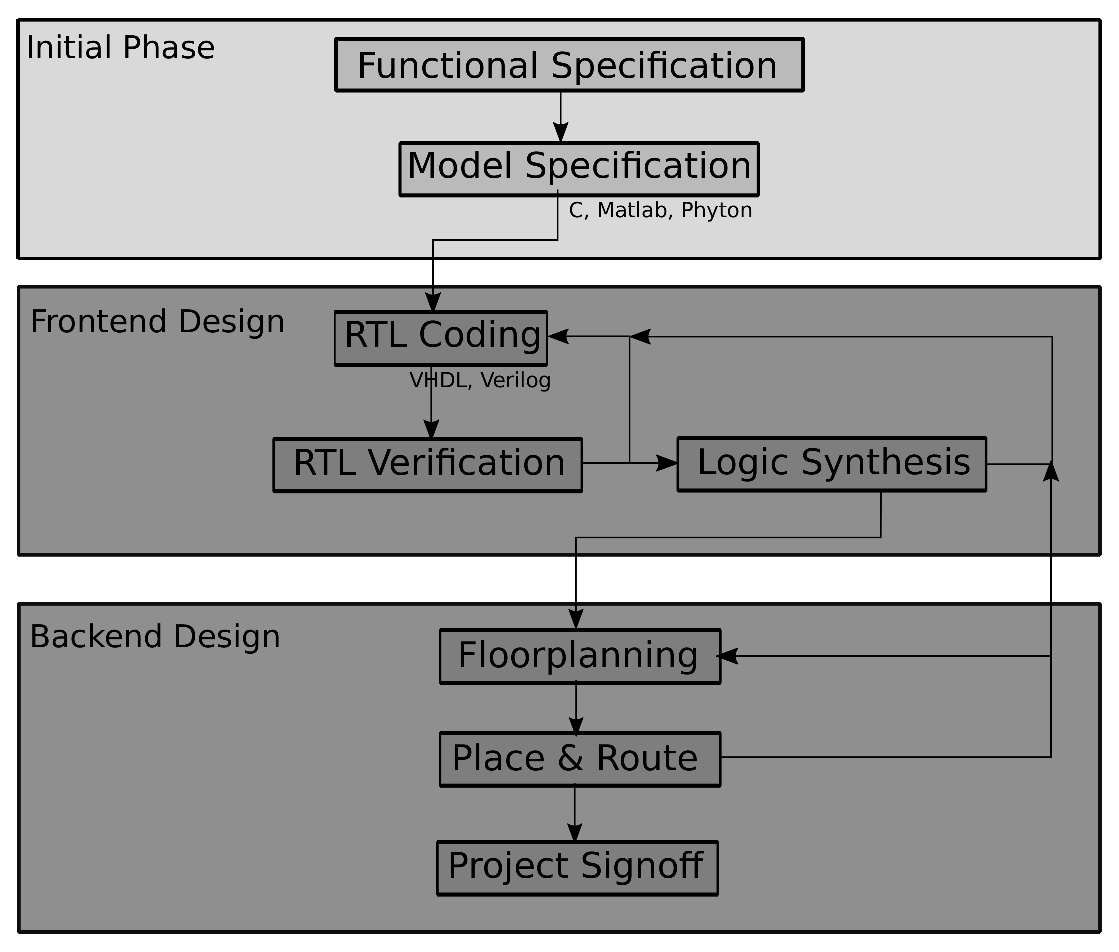
\includegraphics[width=0.6\textwidth]
      {./figures/asic_flow.eps}
%     \rule{35em}{0.5pt}
  \caption{ASIC design flow}
  \label{fig:asic_flow}
\end{figure}

%Once the requirements are defined the architecture is designed. The architecture implements the behavior of the previously defined blocks through boolean functions, finite state machines,
%combinatorial and sequential Logic. That description of the digital circuit is called the Register Transfer Level (RTL), the RTL description or architecture describes a digital circuit that performs complex computations, complex algorithms are described with logic gates, state machines combinational and sequencial logic, as and or gates, multiplexors, . Then, this RTL is described in a Hardware Description Language (HDL), a language developed for digital logic. This description in HDL language goes through a verification process, the behavior of the RTL must match that of the model. 
\section{Front-end}

Once the requirements are defined, the next step is to design the architecture of every block in the system. The architecture is a description of the digital circuit that must perform an intended tasks, also called of Register Transfer Level (RTL), the  digital circuit performs complex computations, protocol management or reorders data. The tasks are described with logic gates, state machines, combinational and sequential logic, \emph{and}, \emph{or} gates, multiplexors and flip flops. After the architecture is completely defined, an RTL description in a Hardware Description Language (HDL) is performed. HDLs describe the structure and behavior of the digital logic circuit, similar to a programming language, it achieves the description by means of a textual description consisting of expressions and statements. 

This RTL behavioral model then goes through a verification process, the behavioral RTL written in HDL language is simulated, and the results are compared with that of the high level language reference model. During the verification process, the circuit is stimulated with real data and timing and functional behavior is tested. The high level language model written in e.g. C, Matlab or Phyton, receives the same stimulus of the behavioral RTL model and generates a reference output. The two outputs are then compared and the RTL debugged if necessary, in case of differences with the reference. Time, behavioral and functional verification at this stage also allows for architectural exploration, optimal data widths (quantization levels) can be adjusted, for blocks involving fixed point computations, and performance issues can be identified.

Once the RTL is verified and no errors are present, Gate Level Synthesis is performed. This synthesis verifies if the HDL description can in fact be mapped to a specific digital hardware. Every logic that is described in the HDL language is mapped onto basic logic gates, \emph{and}, \emph{or} gates and lookup tables, memories and registers are also inferred from the RTL HDL description. Those primitives components are also known as standard cells. The gate level synthesis output is then, a description on a more low level stage. The netlist (the output at this stage) shows an entire structural description of the RTL design. At this stage rough, area, timing and power estimations can be performed, therefore if the goals of the design are not meet e.g. if the maximum frequency of operation defined was 20MHz and the circuit only achieves 15MHz, the behavioral description or even the architecture must be changed in order to attain the time/power/area requirements. 

%yielding estimates that can generate changes in the RTL design. There is a chance in almost all stages of the design, if the timing area or power goal are not reached withing that stage, that it may be necessary to go back to previous stages and modify the design. 

%FPGA prototyping is also performed at this stage, it allows to extend and strengthen ASIC functional verification. Although FPGAs prototypes performance is limited when compared to that of an ASIC, the logical functionality is the same. FPGAs allows for early integration in embedded software and a more realistic verification, since real stimulus can be applied to the design. Another reason to expend time prototyping in FPGA is total development costs, since FPGA prototypes increase the probability of getting the design bug-free in fewer tape-outs. 

FPGA prototyping is also performed at this stage, to extend the design verification. FPGA simulation time is faster than that of a PC allowing less simulation time. Moreover, FPGA prototyping allows for early integration in the embedded system and a more realistic verification, since real stimulus can be applied to the design. Another reason to expend time prototyping in FPGA is total development costs. FPGAs prototypes increase the probability of getting the design bug-free in fewer tape-outs. 

%Although FPGAs prototypes performance is limited when compared to that of an ASIC, the logical functionality is the same. Also, 

\section{Back-end}

Once the frontend bug-free netlist if generated a physical implementation is performed. Basically the process follows three key steps: 

\begin{itemize}
\item \emph{Floor Planing} In Floorplaning the subblocks that compose the design are strategically distributed on the chip area. Blocks are placed in such a way that noise between components is avoided, reduction in timing paths is also 
accomplished and power distribution of the chip is planed.

\item \emph{Placement} The placement process maps the logic with the standard cells and tries to adjust all the cells 
within the chip area to that of the restrictions defined in the floorplaning. The placement process also maps the standard cells to the actual technology used, the pre-designed cells are provided by the foundry (the semiconductor fabrication facility) chosen to manufacture the chip. 

\item \emph{Routing}: Finally the routing process uses the information on the netlist to connect the standard cells one with another. The placement and routing process are iterative, they go back and forth until the process is completed. 

\end{itemize}


After the routing process is complete and timing, function and power requirements are checked, a physical verification is performed. A series of tests are performed on the final circuit: the design rule check (DRC) test some design rules imposed by the foundry, so that the chip can perform as expected. Also, the layout versus schematic (LVS) simulation and an electric rule check (ERC) is performed on the physical verification. 

There is a chance in almost all stages of the ASIC design flow  (if the timing, area or power goals are not reached withing that stage) that it may be necessary to go back to previous stages and modify the design, architecture, RTL (even algorithms can change) if in the final stages the design does not reach the desired results. 

%1. Speed
%2. Area
%3. Power